\subsection{Experimental Setup}\label{subsec:experimental-setup}
%
%推定したい真のvelocity modelは101 x 51のgrid pointsで構成されます.
%初期velocity modelは、真のvelocity modelを標準偏差は80のガウス関数で平滑化したものを使用します.
%source waveletは10 Hzの主周波数を持つRicker waveletを使用します.
%shot数とreceiver数はそれぞれ101と20です.
%勾配Eの計算はdevitoを用いて行われました.
%
%the velocity model is composed of 101 and 51 grid points in the horizontal and vertical directions, respectively.
%We use source wavelet that a Ricker wavelet with a dominant frequency of 10 Hz as the source wavelet.
%number of shots and the receivers are 101 and 20, respectively.
%the initial model obtained by smoothing the velocity model with a Gaussian smoothed function where the standard deviation is 80.
%
To demonstrate the effectiveness of the TV and box constrained FWI, we conducted experiments where we compared with the normal FWI with gradient method~\eqref{eq:FWIWithGradient}, using the SEG/EAGE Salt and Overthrust Models.
The velocity model consists of 101 $\times$ 51 grid points, and the initial velocity model is generated by smoothing the true velocity model with a Gaussian function with a standard deviation of 80.
Number of receivers and source shots are 101 and 20, respectively.
The source waveform is a Ricker wavelet with a peek wavelet frequency of 10 Hz.
The gradient of $E$ is computed numerically using the Devito framework\cite{devito}.
In normal FWI, the step size $\gamma$ is set to $1.0 \times 10^{-4}$.
In TV and box constrained FWI, the step size $\gamma_1$ and $\gamma_2$ are set to $1.0 \times 10^{-4}$ and $1.0 \times 10^2$, respectively, the upper bound of the $l_{1,2}$ norm $\alpha$ is set to 400 and the lower and upper bounds of the velocity model $a$, $b$ are set to 1.5[km/s] and 4.5[km/s], respectively.
Number of iterations is set to 5000.


\begin{figure*}[htbp]
    \centering
    \begin{tabular}{m{68mm} m{70mm} m{10mm}}
        % First row: Image 1, 2, and vertically spanning Image 5
        \begin{minipage}[b]{70mm}
            \centering
            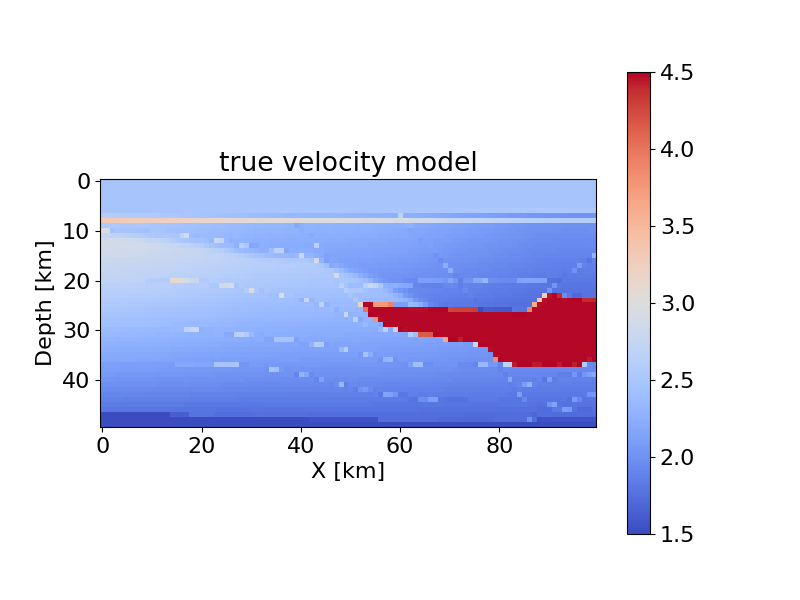
\includegraphics[width=70mm]{public/true}
            \caption*{\raisebox{5mm}{Background truth}}
        \end{minipage} &
        \begin{minipage}[b]{70mm}
            \centering
            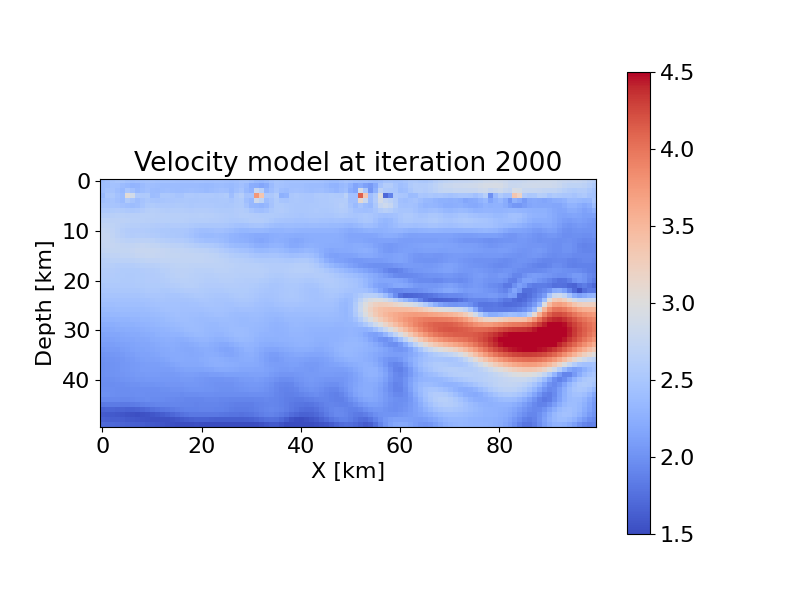
\includegraphics[width=70mm]{public/gradient}
            \caption*{\raisebox{5mm}{Reconstructed with normal FWI}}
        \end{minipage} &
        \multirow[t]{2}{*}{\raisebox{-50mm}{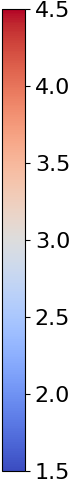
\includegraphics[height=68mm]{public/color-bar}}} \\
        % Second row: Image 3 and 4
        \begin{minipage}[b]{70mm}
            \centering
            
\includegraphics[width=70mm]{public/initial}
            \caption*{Initial model}
        \end{minipage} &
        \begin{minipage}[b]{70mm}
            \centering
            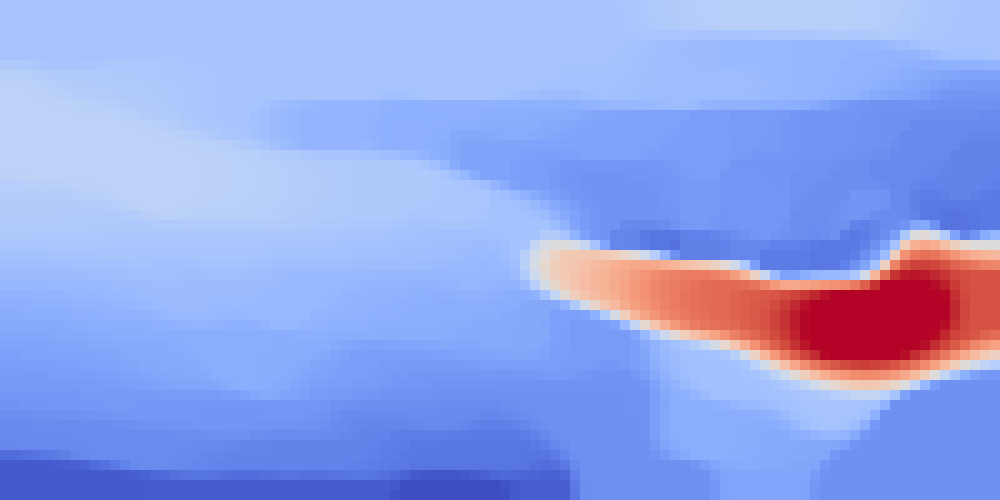
\includegraphics[width=70mm]{public/pds}
            \caption*{Reconstructed with the constrained FWI}
        \end{minipage} &
    \end{tabular}
    \caption{Velocity models and their corresponding reconstructions.}
    \label{fig:velocity-models}
\end{figure*}



\subsection{Results and Discussion}\label{subsec:results-and-discussion}

Table 1 presents a summary of the restoration performance achieved by DnCNN-PnP-PDS and other methods.
Across all tasks, we rec- ognize that our proposed DnCNN-PnP-PDS has achieved restoration performance comparable to that of DnCNN-PnP-FBS.
We remark again that the proposed approach simplified parameter tuning when compared to DnCNN-PnP-FBS.
Specifically, in this experiment, we √ rewrite the parameter ε in (9) by α ∈ R as follows: ε = ασ K.
√ Note that σ sian noise with the variance σ.
The value of α in DnCNN-PnP-PDS was set to 0.
5 for all cases, whereas λ in (10) varied from task to task for DnCNN-PnP-FBS.
Additionally, we experimentally found that in deblurring, the appropriate λ value was higher than in inpainting.

\begin{figure}[htbp]\label{fig:ssim}
\vspace{-\baselineskip}
\begin{center}
    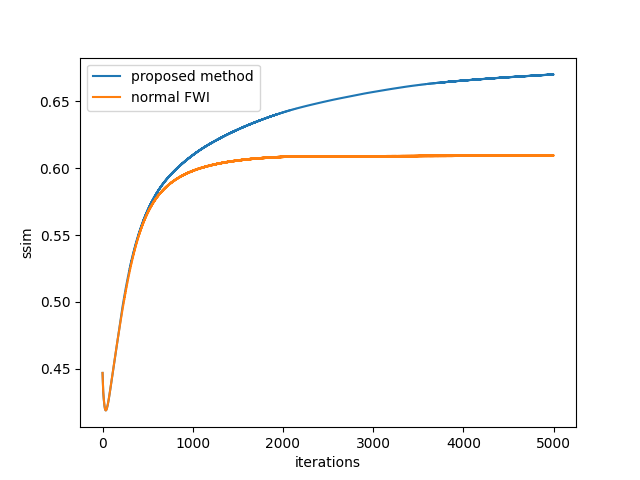
\includegraphics[width=80mm]{public/ssim}
    \caption{ssim}
\end{center}
\vspace{-\baselineskip}
\end{figure}







